\Section{Evaluation}
\label{VT:Sec:Experiments}

In this section, we give experimental results to validate our implementation of the virtual time supported Mininet-Hifi network emulator.
Very straightforward but nontrivial network typologies are adopted to demonstrate
that the emulation system described in~\ref{VT:Sec:Implementation} can improve fidelity, scalability as well as efficiency. 

All the experiments are conducted on a Dell XPS 8700 Desktop with one Intel Core i7-4790 CPU,
12 GB RAM and one gigabit Ethernet interface. The machine runs a 64-bit Ubuntu 14.04.1 LTS with our customized 3.16.3 Linux kernel.
The benchmark scores of this machine's CPU and FPU are: 1.52 seconds for Blowfish, 1045.62 MiB/seconds for CryptoHash,
0.63 seconds for FFT and 2.56 seconds for Raytracing. Our virtual-time-enabled Mininet was built on the latest version of Mininet (2.1.0),
also named Mininet-Hifi, at the time of development.

\Subsection{Fidelity}
We first evaluate how our virtual time system improves Mininet's fidelity through a basic network scenario:
a single TCP flow transmission through a chain of switches in an emulated SDN network.
As shown in Figure~\ref{VT:Fig:ChainTopoExample}, the network topology consists of a client-server pair connected by a chain of Open vSwitch switches in Mininet.
We setup the default OpenFlow controller to function as a learning switch.
In this set of experiments, we connected two hosts through 40 switches in Mininet, and all the links are configured with 10 $\mu s$ delay.
We used \texttt{iperf3}~\cite{iperf3} to generate a TCP flow between the client and the server.
TDF was set to 1 (i.e., no virtual time) and 4 for comparison. We also setup a real testbed for ``ground truth" throughput data collection.
The testbed was composed of two machines connected by a 10 Gbps Ethernet link.
We varied the bandwidth link from 100 Mbps to 10 Gbps and measured the throughput using \texttt{iperf3}.
In the real testbed, we manually configured the link bandwidth and delay using \texttt{tc},
and the delay was set as the corresponding round trip times (RTTs) measured in the switch chain topology in Mininet,
so that the networking settings were tightly coupled for comparison.
Although we did not setup an exact network with SDN switches,
the stabilized TCP throughputs generated by the physical testbed should reflect what occurs in a real SDN network.
Each experiment was repeated 10 times and the results with bandwidth 4 Gbps, 8 Gbps and 10 Gbps were reported in Figure~\ref{VT:Fig:Perf40SwDiffBw}. 

We observe that when the bandwidth was no greater than 4 Gbps (we only displayed the 4 Gbps case in the figure),
Mininet was able to accurately emulate the TCP flow with and without virtual time,
as the average throughputs were very close to the ones collected from the physical testbed.
However, when we continued to increase the bandwidth, Mininet was not able to produce the desired throughputs, e.g.,
28\% (8 Gbps) and 39\% (10 Gbps) smaller than the physical testbed throughputs.
With virtual time (TDF = 4), Mininet was capable to accurately emulate the TCP flow even at high bandwidth,
and the results were nearly the same as the ones measured in the physical testbed. 

The root cause is that the machine running Mininet does not have sufficient resources to emulate networks with bandwidth greater than 4 Gbps,
which would lead to fidelity issues, e.g., low expected throughputs.
Note that we only emulated a single flow, and the results could be much worse and unpredictable in complicated multi-flow scenarios.
Results show that virtual time can significantly enhance the performance fidelity
by ``slowing down" the experiments so that the system has sufficient resources and time to correctly process the packets.
We further illustrate the effect by plotting the time series of throughput changes for the 10 Gbps cases in Figure~\ref{VT:Fig:Perf40Sw10GbLink}.
With virtual time, the throughputs measured in Mininet closely match the real testbed results;
without virtual time ($TDF = 1$), the ramp up speed was much slower, in particular,
22 seconds ($TDF = 1$) rather than 4 seconds ($TDF = 4$), and the throughput was incorrectly stabilized below 6.1 Gbps.

\Subsection{Scalability}
Virtual time also improves the scale of networks that one can emulate without losing fidelity.
In this set of experiments, we used the same switch chain topology in Figure~\ref{VT:Fig:ChainTopoExample},
and set the link bandwidth to 4 Gbps. We want to investigate, with virtual time,
how many switches Mininet is capable to emulate without losing fidelity, i.e., preserving nearly 4 Gbps throughput.
This time we increased the number of switches with the following values \texttt{\{20, 40, 60, 80, 100\}},
and TDF was selected to be 1 (no virtual time) and 4. We ran \texttt{iperf3} for 25 seconds between the client and the server.
Each experiment was repeated ten times, and the throughput measurement is reported in Figure~\ref{VT:Fig:ScaleDiffSw4GbLink}.

In the case of $TDF = 1$, the average throughput kept decreasing as the number of switches grew over 20.
The throughput decreased dramatically when the number of switches was greater than 60 (e.g., decreased by 41\% for 60 switches, 65\% for 80 switches, and 83\% for 100 switches).
The standard deviation, indicated the undesired high disturbance, also grew as number of switches increased.
When virtual time was applied with $TDF = 4$, the throughput was always around 3.8 Gbps with small standard derivations in all the experiments.
It is clear that virtual time helps to scale up the emulation.
In this case, Mininet can emulate 100 switches with 4 Gbps links and still generate the accurate throughputs,
rather than being saturated at 20 switches without virtual time. 

We also recorded the running time in Figure~\ref{VT:Fig:ScaleTime}.
Longer execution time is the tradeoff for the fidelity and scalability improvement.
When $TDF=4$, the execution time was about 4 times longer than the time required in the case of $TDF=1$ in all the experiments.
In fact, we have conducted extensive experiments with different TDF values on multiple network scenarios.
The general observation is that a larger TDF allows an emulator to conduct accurate experiments with larger scale on the same physical machine,
but typically requires longer execution time, approximately proportional to the TDF.
This leads to the question on how to balance the speed and fidelity,
and our approach is to explore the adaptive time dilation scheduling, whose evaluation is presented in the next section. 

\begin{figure}
    \centering
    \subfigure[Chain Network Topology]{{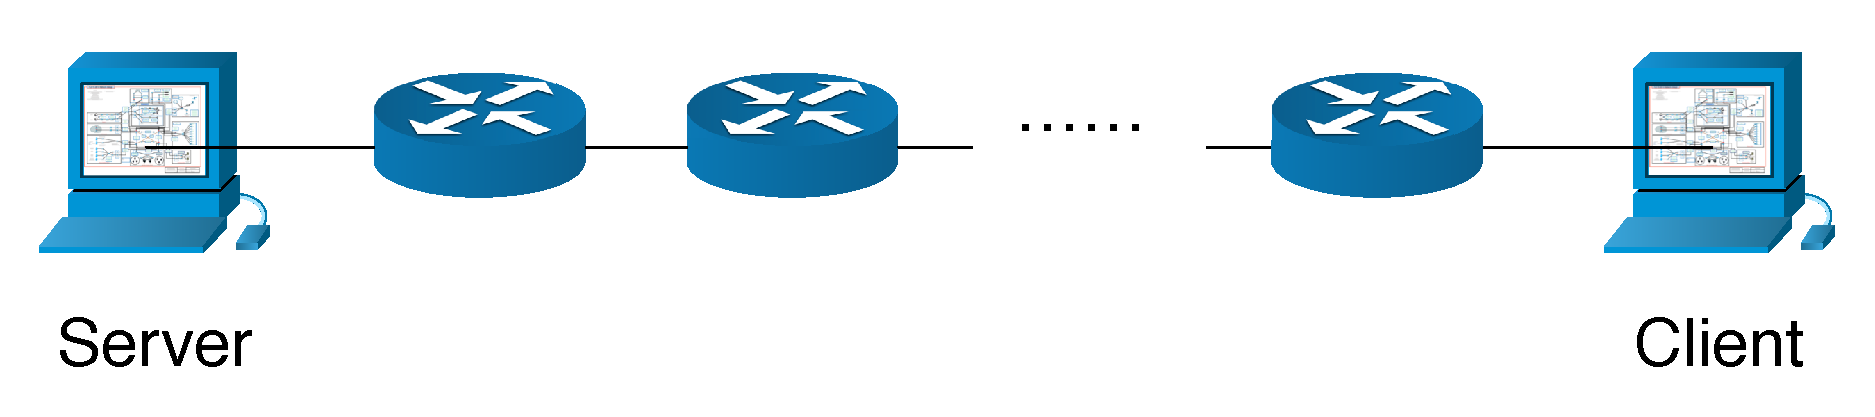
\epsfig{file=VirtualTime/figures/TopoChainExample.eps, width=0.45\textwidth}}
    \label{VT:Fig:ChainTopoExample}}
    \subfigure[Linear Network Topologies]{{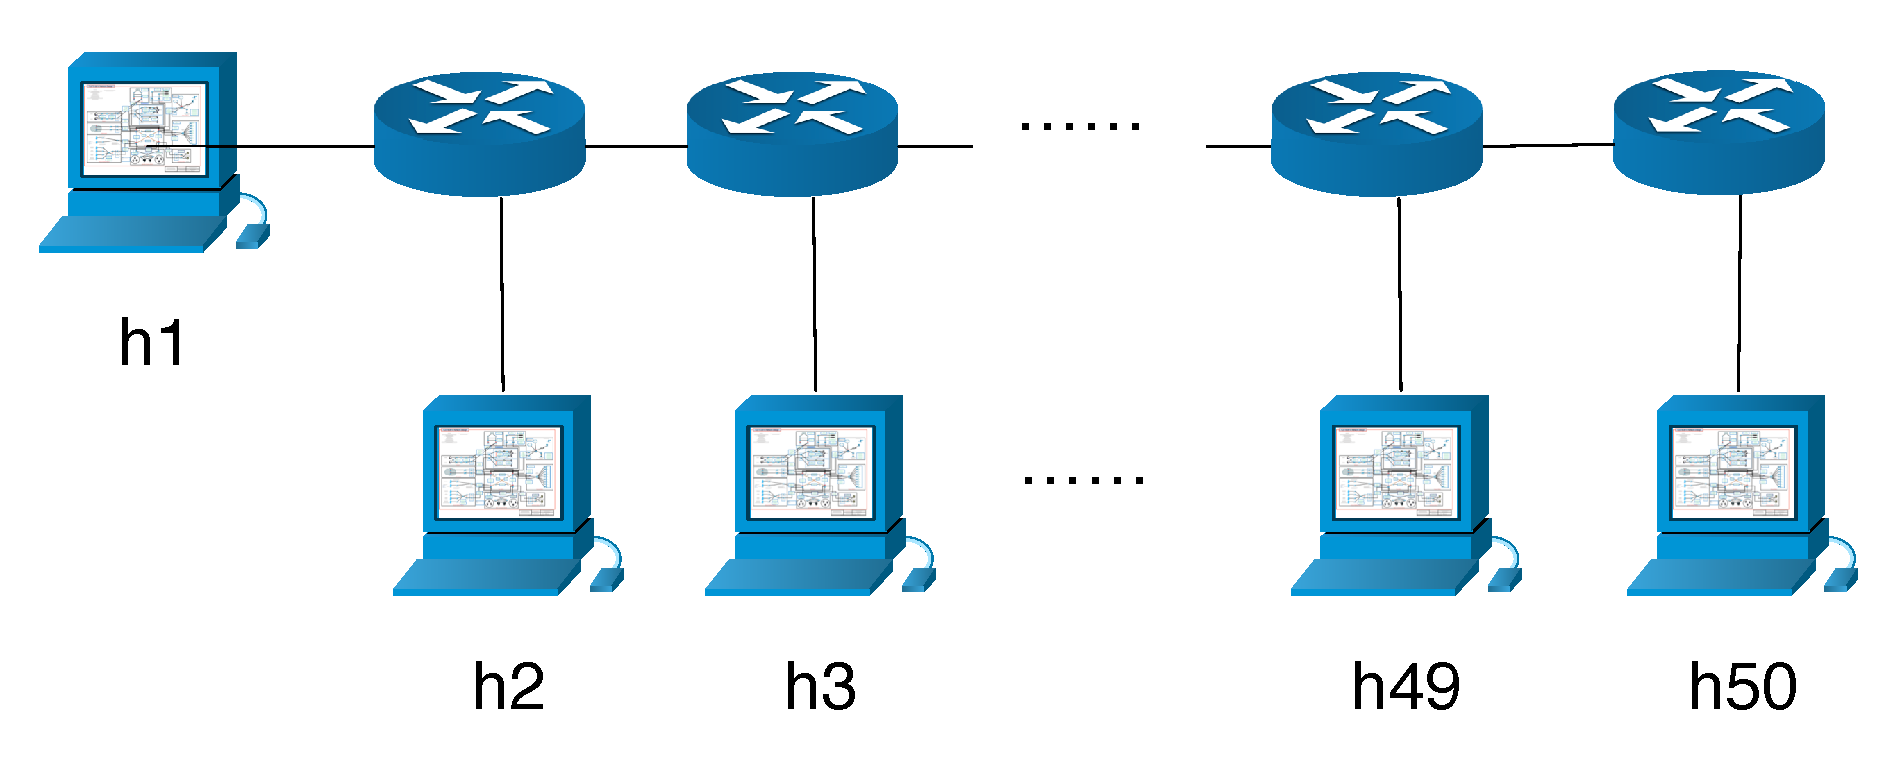
\epsfig{file=VirtualTime/figures/TopoLinearExample.eps, width=0.45\textwidth}}
    \label{VT:Fig:LinearTopoExample}}
    \caption{Network Topologies Used in Virtual Time Evaluation}
\end{figure}

\begin{figure}[t]
    \centering
    \subfigure[TCP Throughput with Different Link Bandwidths]{{\epsfig{file=VirtualTime/figures/Perf40SwDiffBw.eps, width=0.45\textwidth}}
    \label{VT:Fig:Perf40SwDiffBw}}
    \subfigure[TCP Throughput with 10 Gbps Links]{{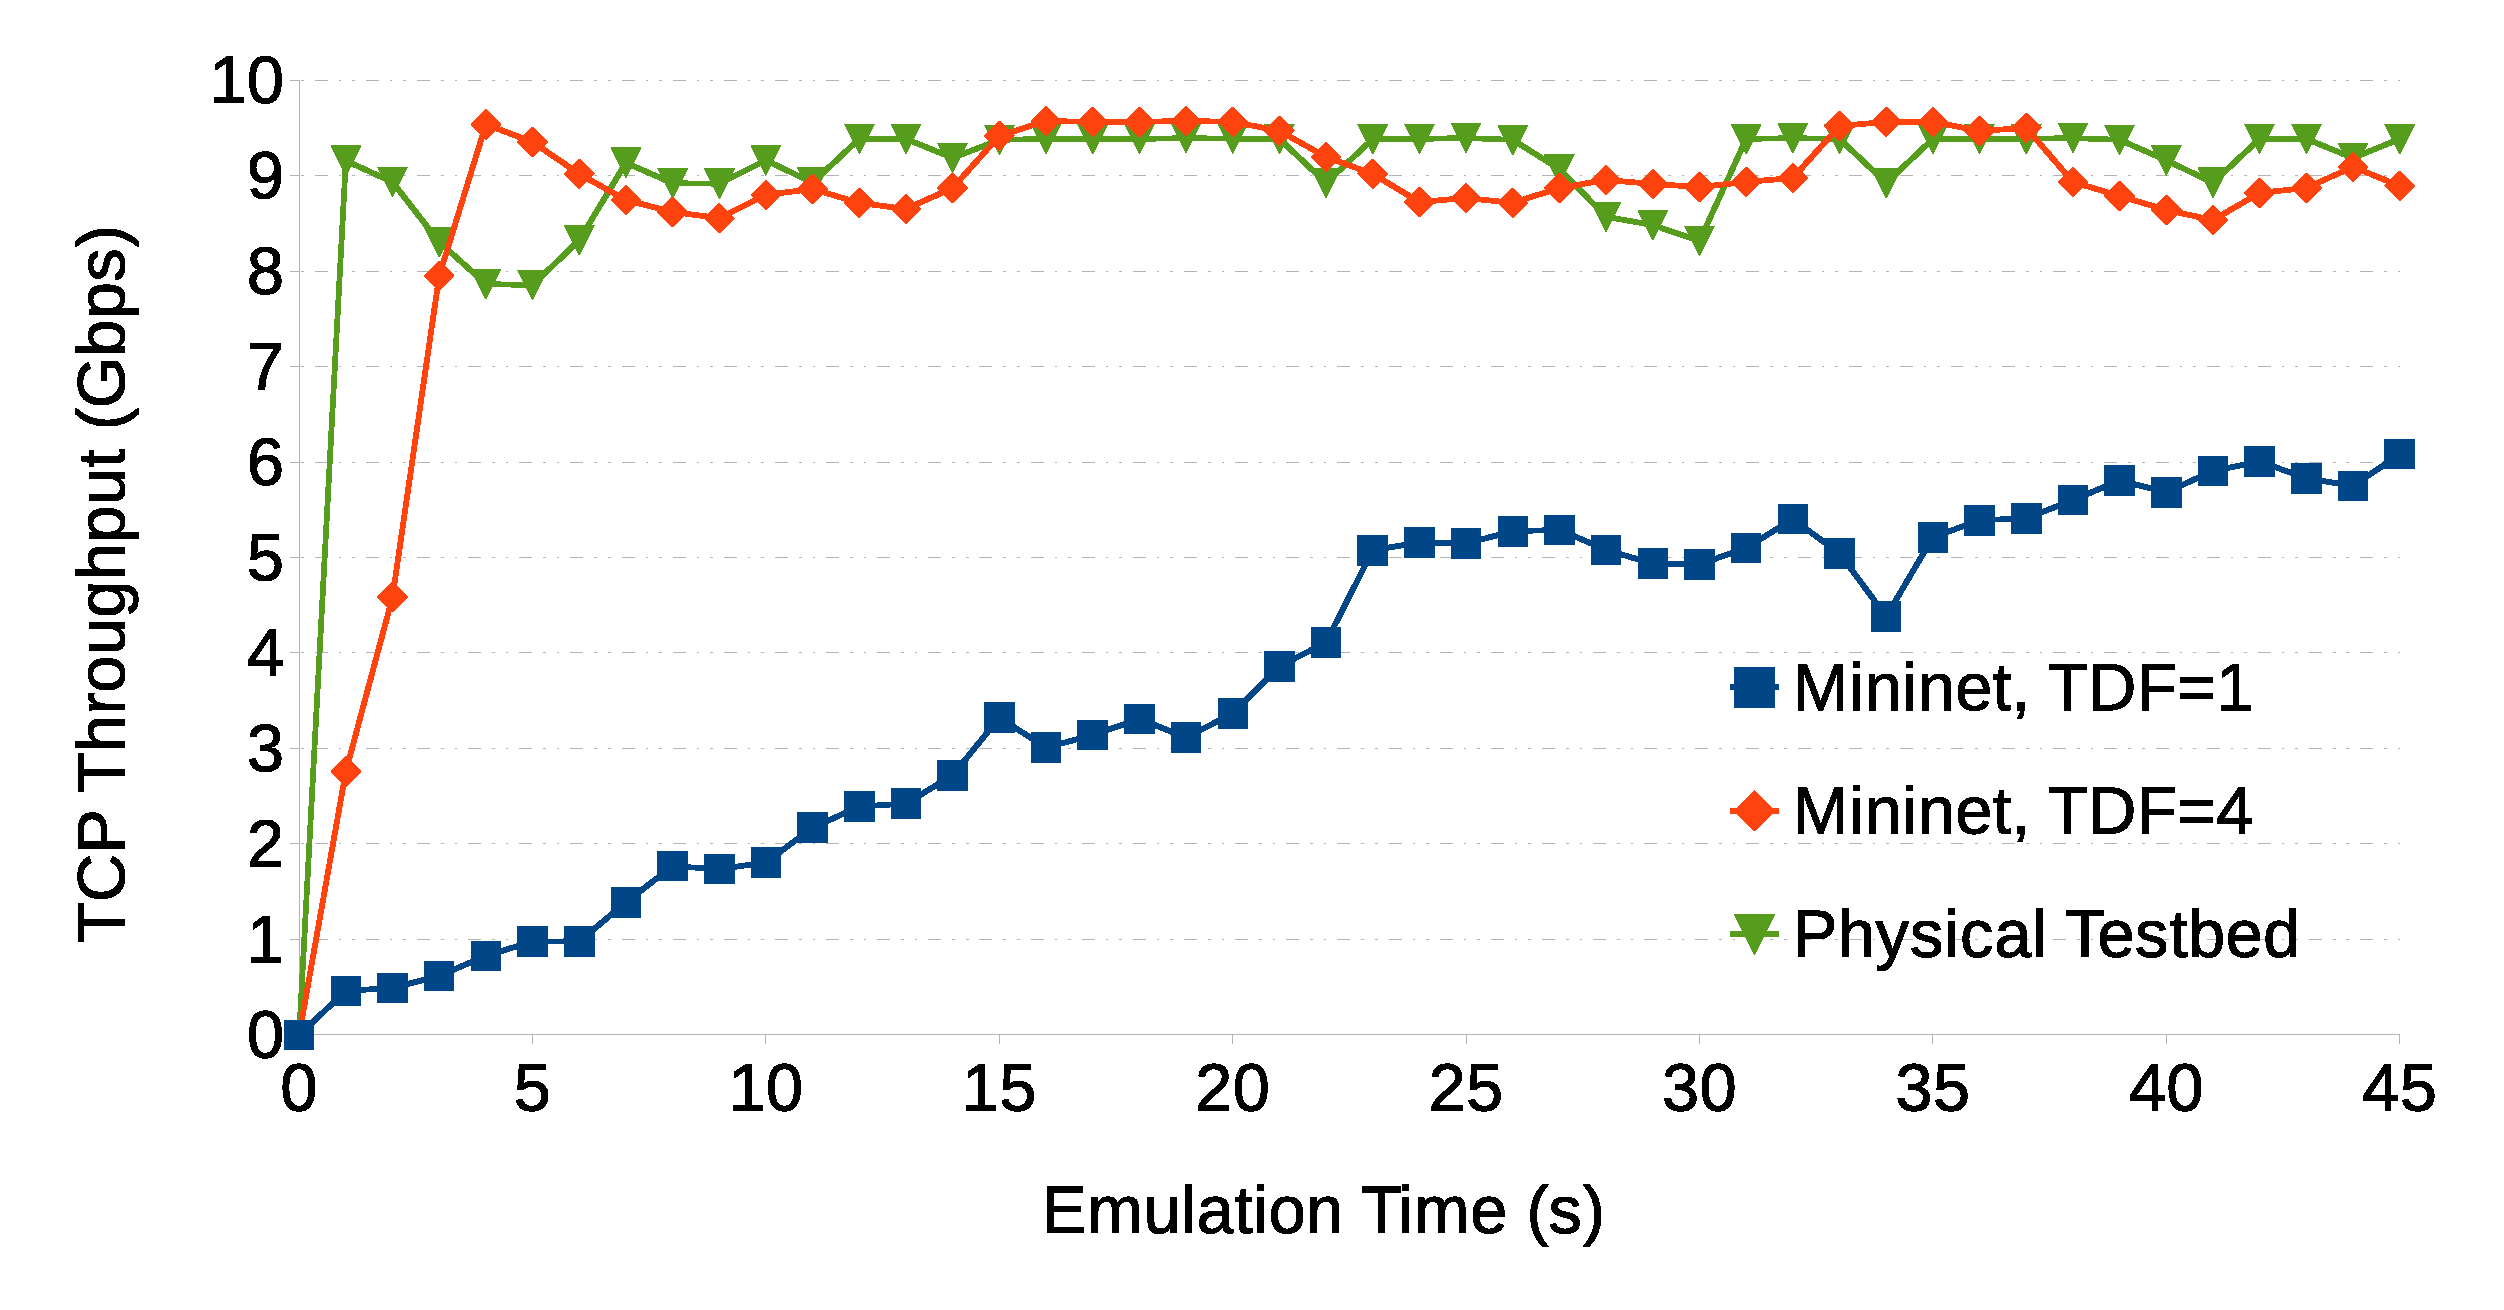
\epsfig{file=VirtualTime/figures/Perf40Sw10GbLink.eps, width=0.45\textwidth}}
    \label{VT:Fig:Perf40Sw10GbLink}}
    \caption{Fidelity Evaluation Experimental Results}
\end{figure}

\begin{figure}[t]
    \centering
    \subfigure[TCP Throughput]{{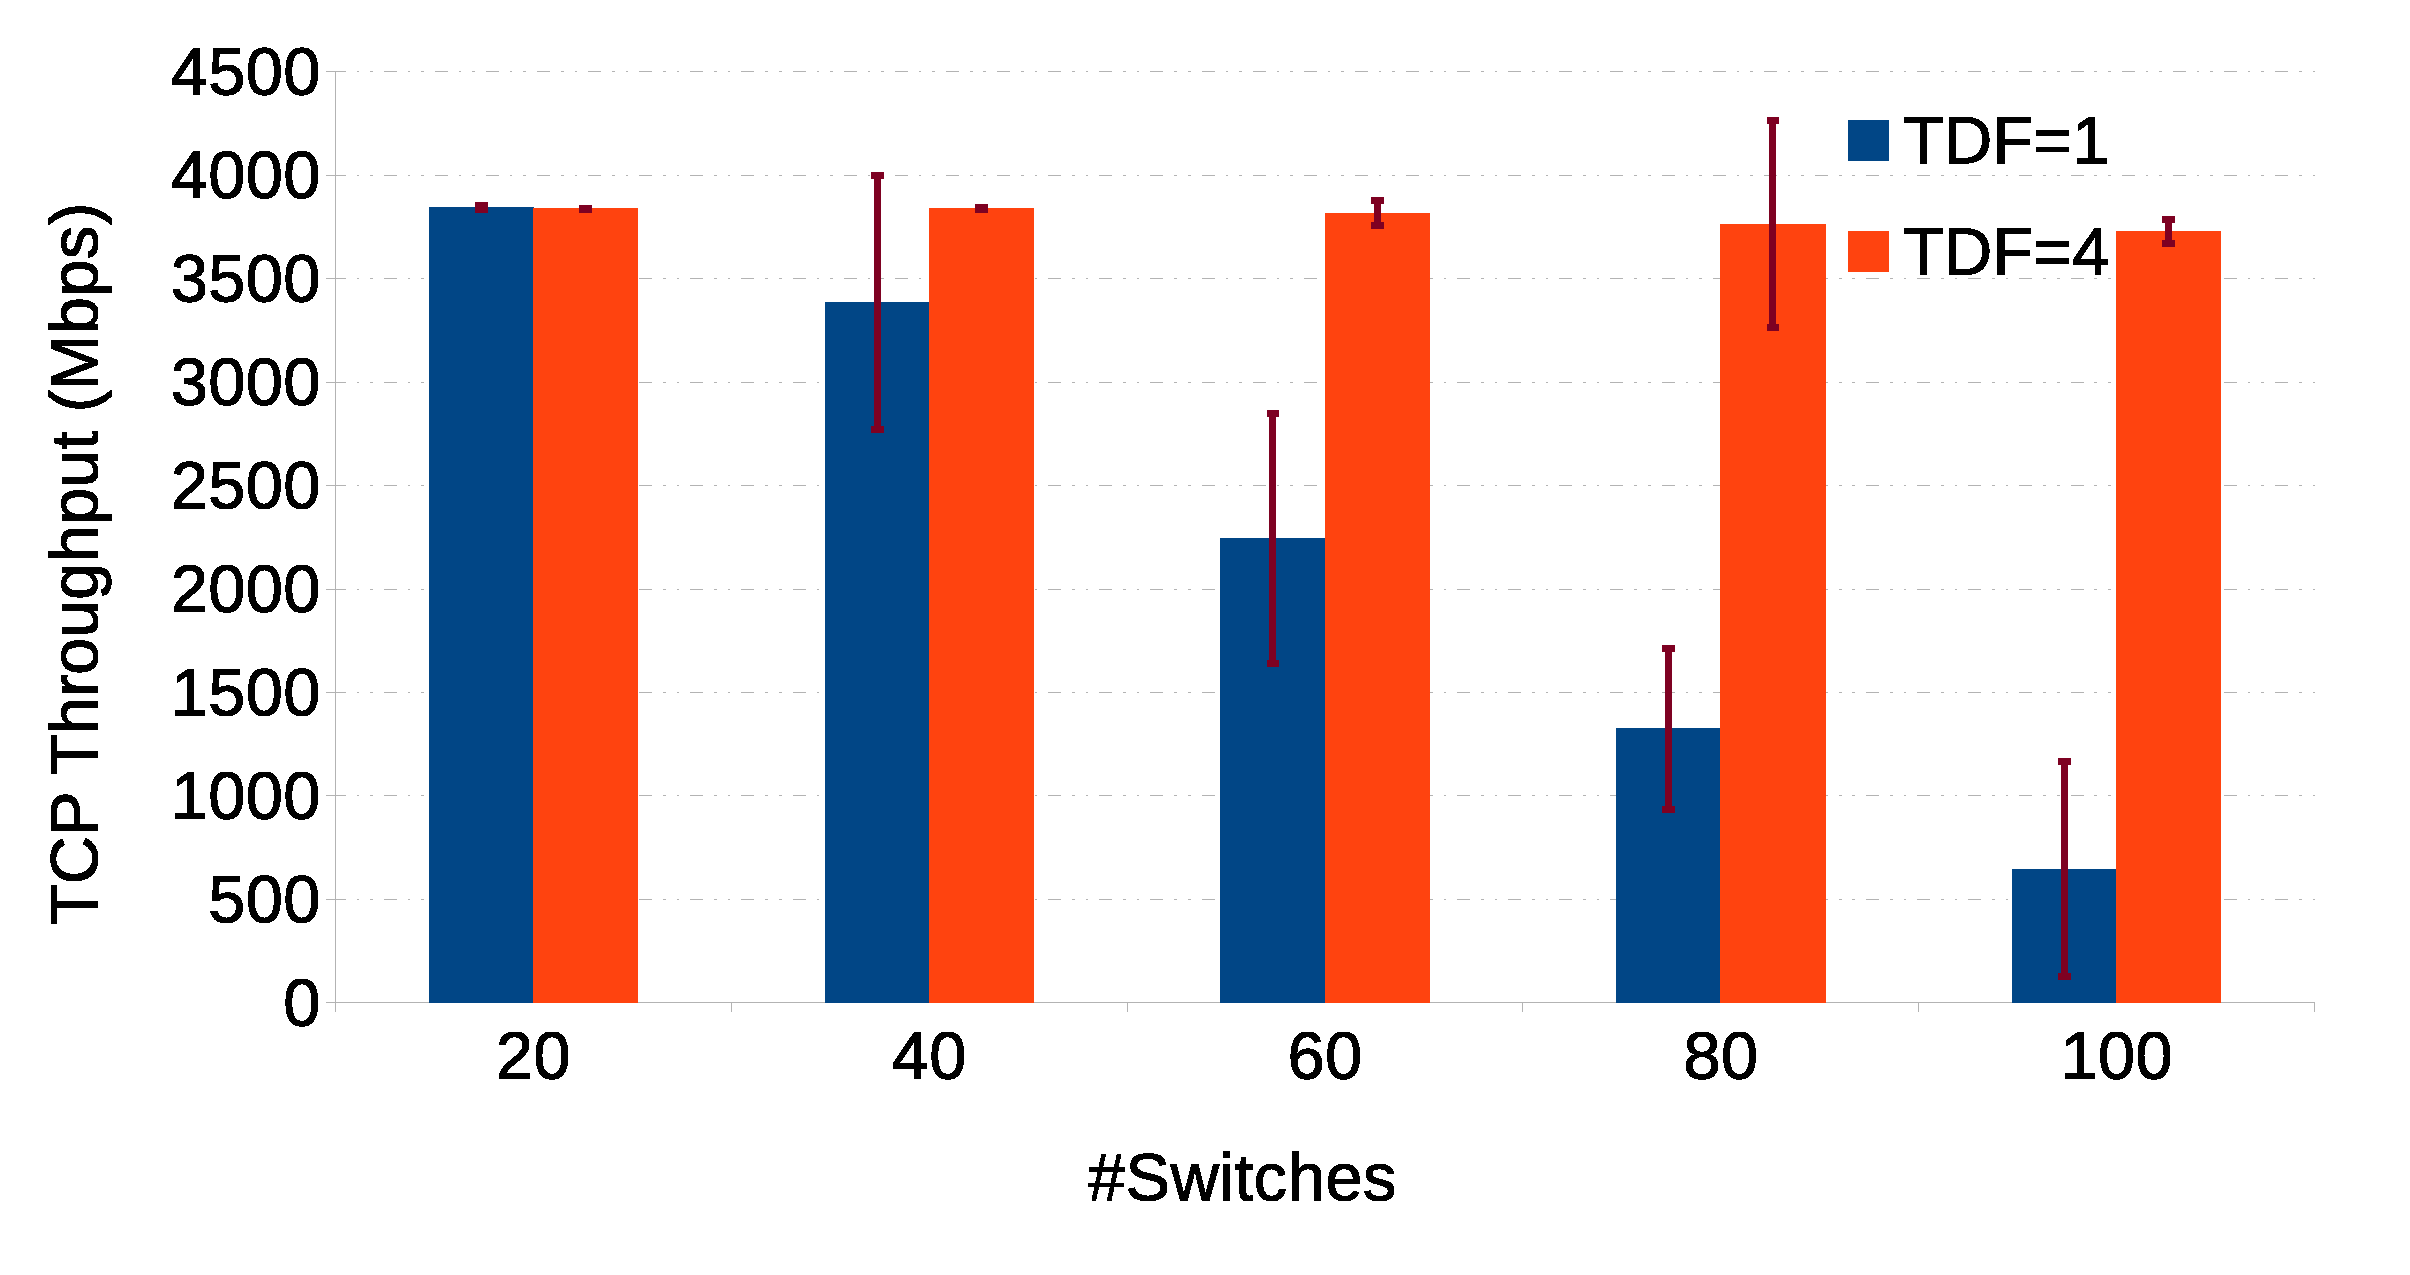
\epsfig{file=VirtualTime/figures/ScaleDiff100Sw4GbLink.eps, width=0.45\textwidth}}
    \label{VT:Fig:ScaleDiffSw4GbLink}}
    \subfigure[Evaluation Running Time]{{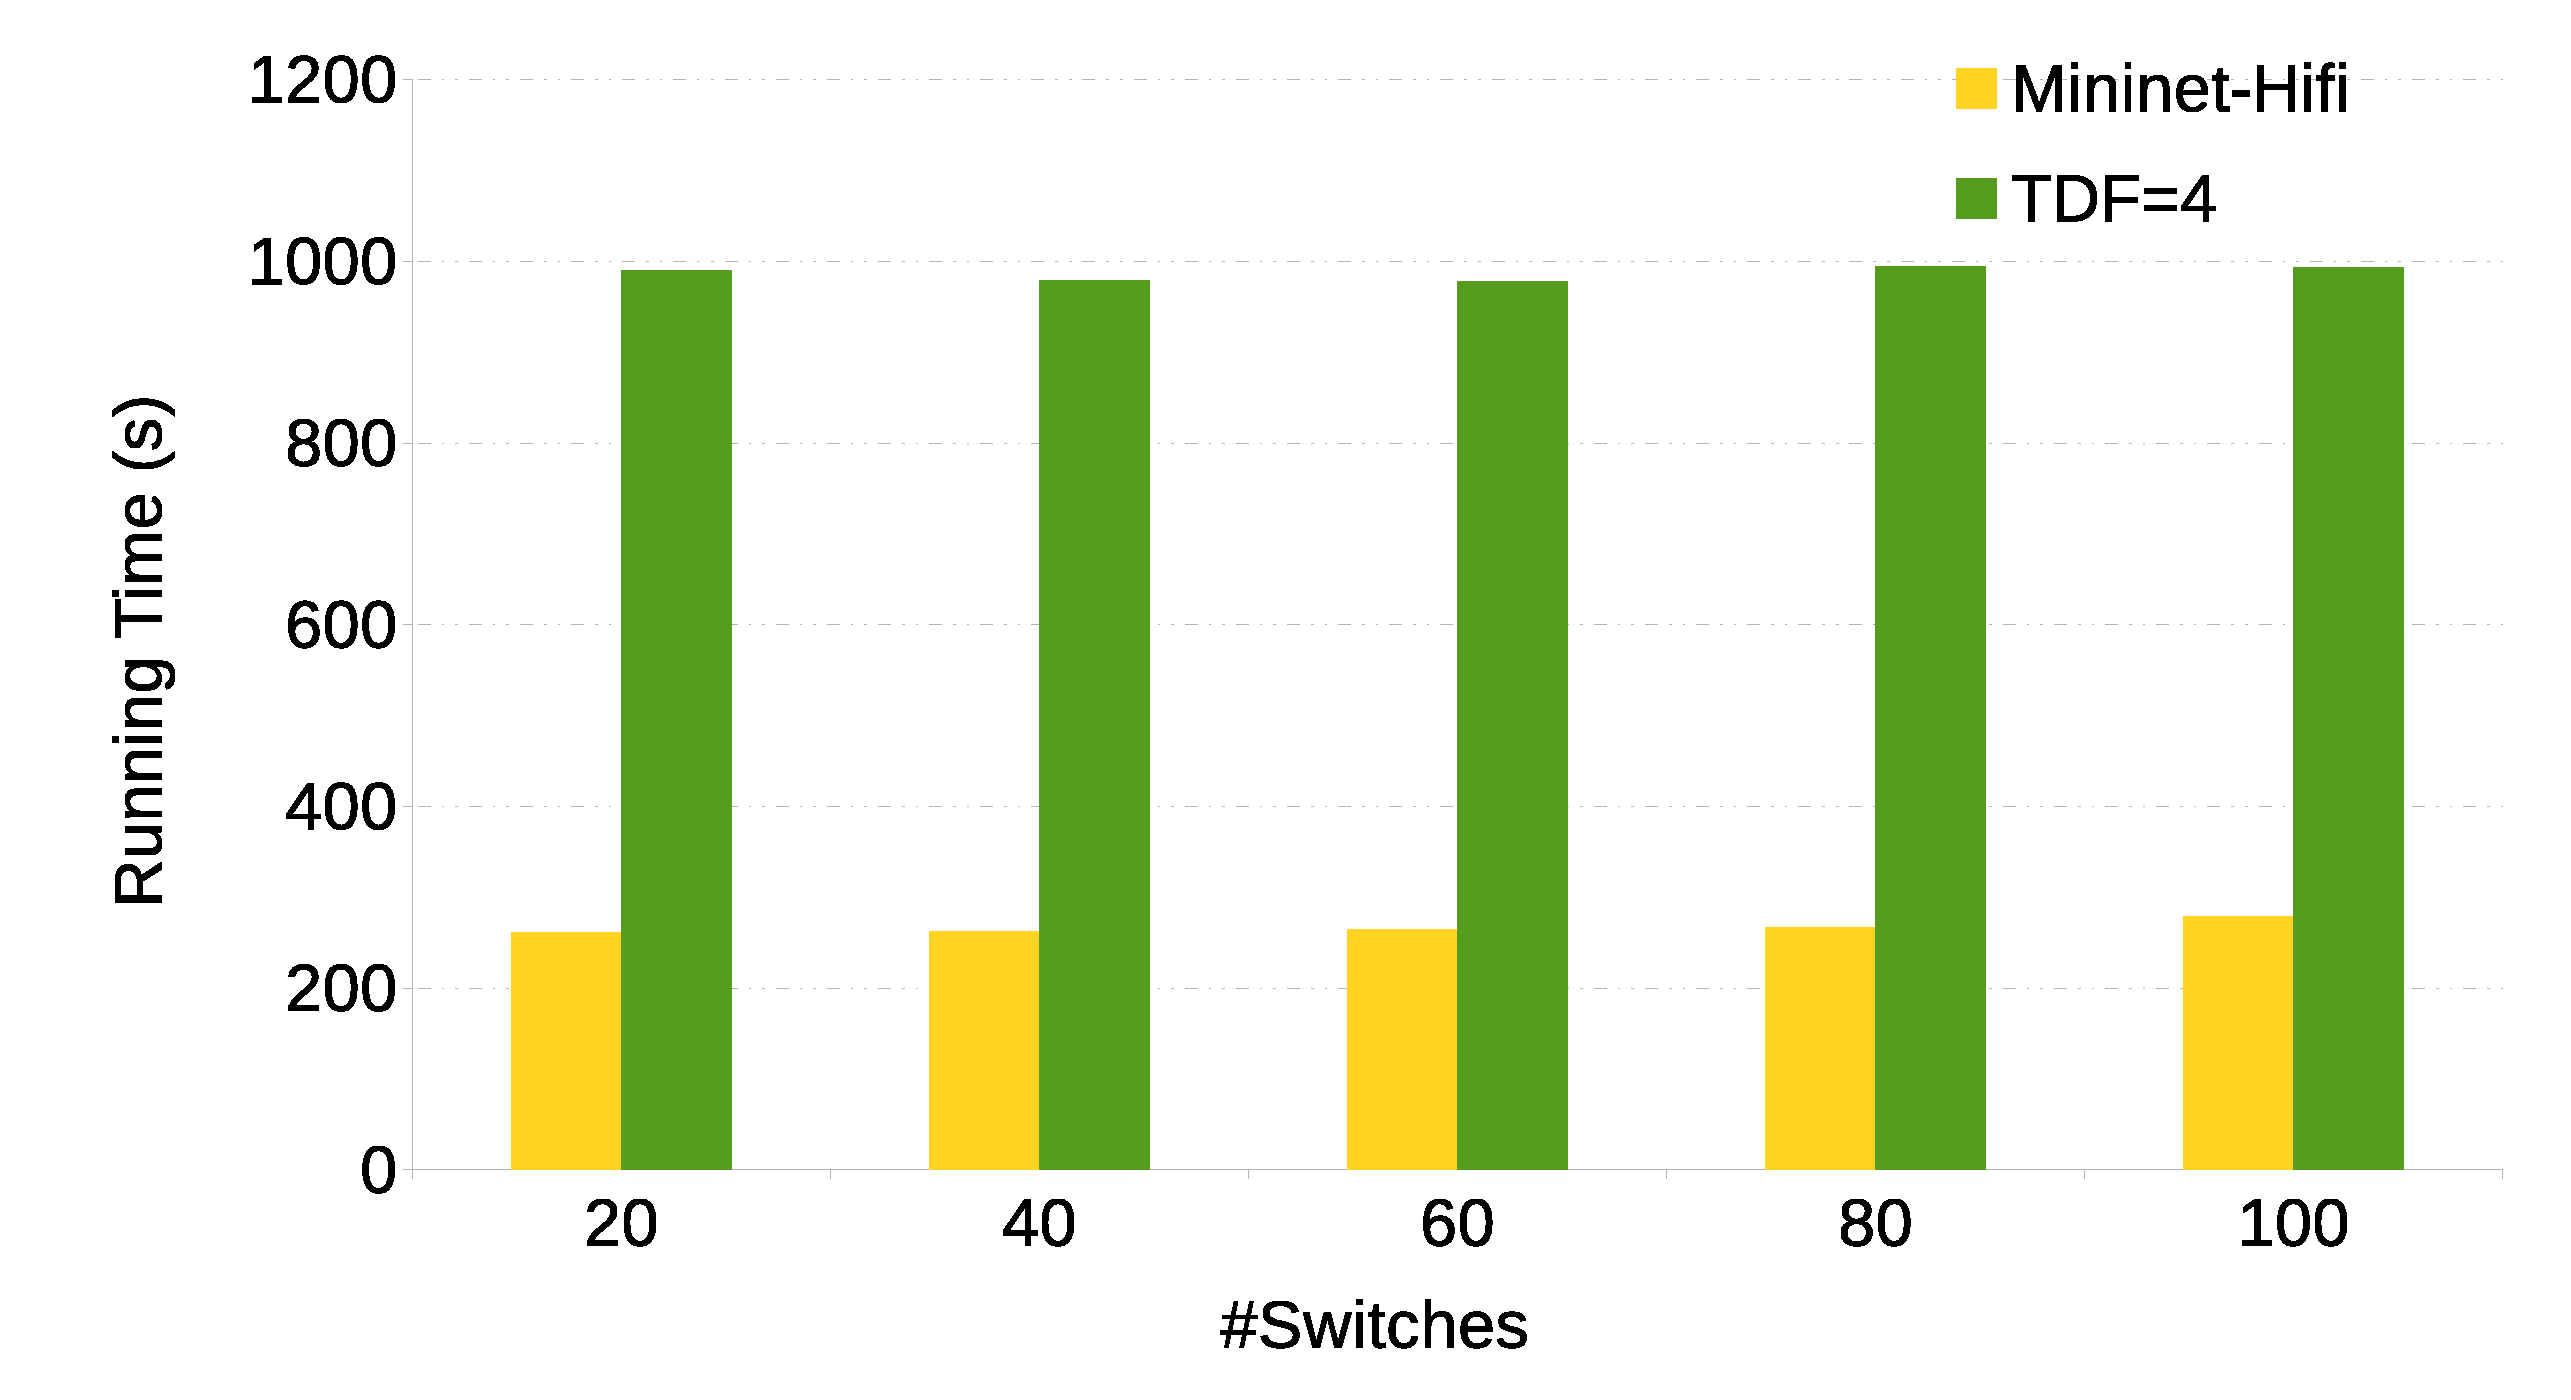
\epsfig{file=VirtualTime/figures/ScaleTime100Sw4GbLink.eps, width=0.45\textwidth}}
    \label{VT:Fig:ScaleTime}}
    \caption{Scalability Evaluation Experimental Results}
\end{figure}

\Subsection{Adaptive TDF Scheduling}
We design a set of emulation experiments consisting of multiple TCP flows to evaluate the adaptive TDF scheduling algorithm.
The network topology has a simple linear structure as shown in Figure~\ref{VT:Fig:LinearTopoExample} and consists of 100 hosts and 99 switches.
All the links are of 100 Mbps bandwidth and 1 ms delay.
We selected 5 non-overlap client-server pairs: \texttt{(h1, h20), (h21, h40), h(41, h60), h(61, h80), (h81, h100)}.
The entire experiment was divided into three phases: (1) initially, transmit flow \texttt{(h1,h20)},
(2) after 50 seconds, transmit all five flows, and (3) after 150 seconds, stop all the transmissions except for flow \texttt{(h1,h20)}.
The goal is to evaluate how our adaptive time dilation scheduler behaves under dynamic emulation workloads with the peak load exceeding Mininet's capability.

We ran the experiments in three cases.
In case 1, TDF was set to 1 (i.e., no virtual time) and the adaptive virtual time scheduling was disabled.
All flows' TCP throughputs measured by \texttt{iperf3} over time are plotted in Figure~\ref{VT:Fig:5FlowsNoVT}. 
In case 2, we enabled the adaptive time dilation management system with TDF initially set to 1,
and conducted the same emulation experiments. Figure~\ref{VT:Fig:5FlowsAdaptiveVT} plots the throughputs of all five flows.
In case 3, we used a fixed TDF ($TDF = 11$) and disabled the adaptive virtual time scheduling.
Results are shown in Figure~\ref{VT:Fig:5FlowsFixedVT}.
We set $TDF=11$ because 11 was the largest value observed in the TDF changing history in case 2.
In addition, the entire trace of the dynamic TDF in case 2 is plotted in Figure~\ref{VT:Fig:HistoryTDF}.
We repeated each experiment for 5 times and observed very similar behaviors.
All the time series reported in Figure~\ref{VT:Fig:Adaptive} were based on the data collected from one run. 

In phase 1, Mininet had sufficient system resources to emulate a single TCP flow \texttt{(h1, h21)}.
Therefore, we observe the close-to-line-rate throughput, i.e., 100 Mbps, in all three cases.
In phase 2, there were five concurrent flows in the network and each case demonstrated different behaviors.
Note that those flows were non-overlap flows because they did not share any links or switches.
Therefore, all five flows should achieve close-to-line-rate throughputs, i.e., 100 Mbps, in physical world applications.
In case 1, the throughputs of all five flows were very unstable as shown in Figure~\ref{VT:Fig:5FlowsNoVT},
which reflected the heavy resource contention in Mininet.
In contrast, in case 3, all five flows have stable, close-to-100-Mbps throughputs because of the virtual time.
In case 2, we observed disturbances in throughput at the beginning of phase 2,
but the five flows quickly converged to the stable close-to-line-rate throughput because the adaptive TDF scheduler managed to compute the optimal TDF value.
The details of TDF adjustment are depicted in Figure~\ref{VT:Fig:HistoryTDF}.
In phase 3, the emulation returned back to a single flow \texttt{(h1, h21)}, and the measured throughputs were accurate in all three cases.
As indicated by Figure~\ref{VT:Fig:HistoryTDF}, our scheduler decreased the TDF value accordingly
in case 2 to save emulation time in phase 3 while still preserving the fidelity.

Table~\ref{VT:Tab:CompareRunTime} summarizes the execution time, the average TDF,
and the rate of execution time in wall clock to the emulation time (200 seconds) of all three cases. 
We can see that case 3 ($TDF = 11$) is around 10 times slower than case 1 ($TDF = 1$) in order to guarantee fidelity.
Our adaptive time dilation scheduler managed to reduce 46\% of the running time as compared to case 3 with little fidelity loss. 

\begin{figure}[t]
    \centering
    \subfigure[TCP Throughput without Virtual Time]{{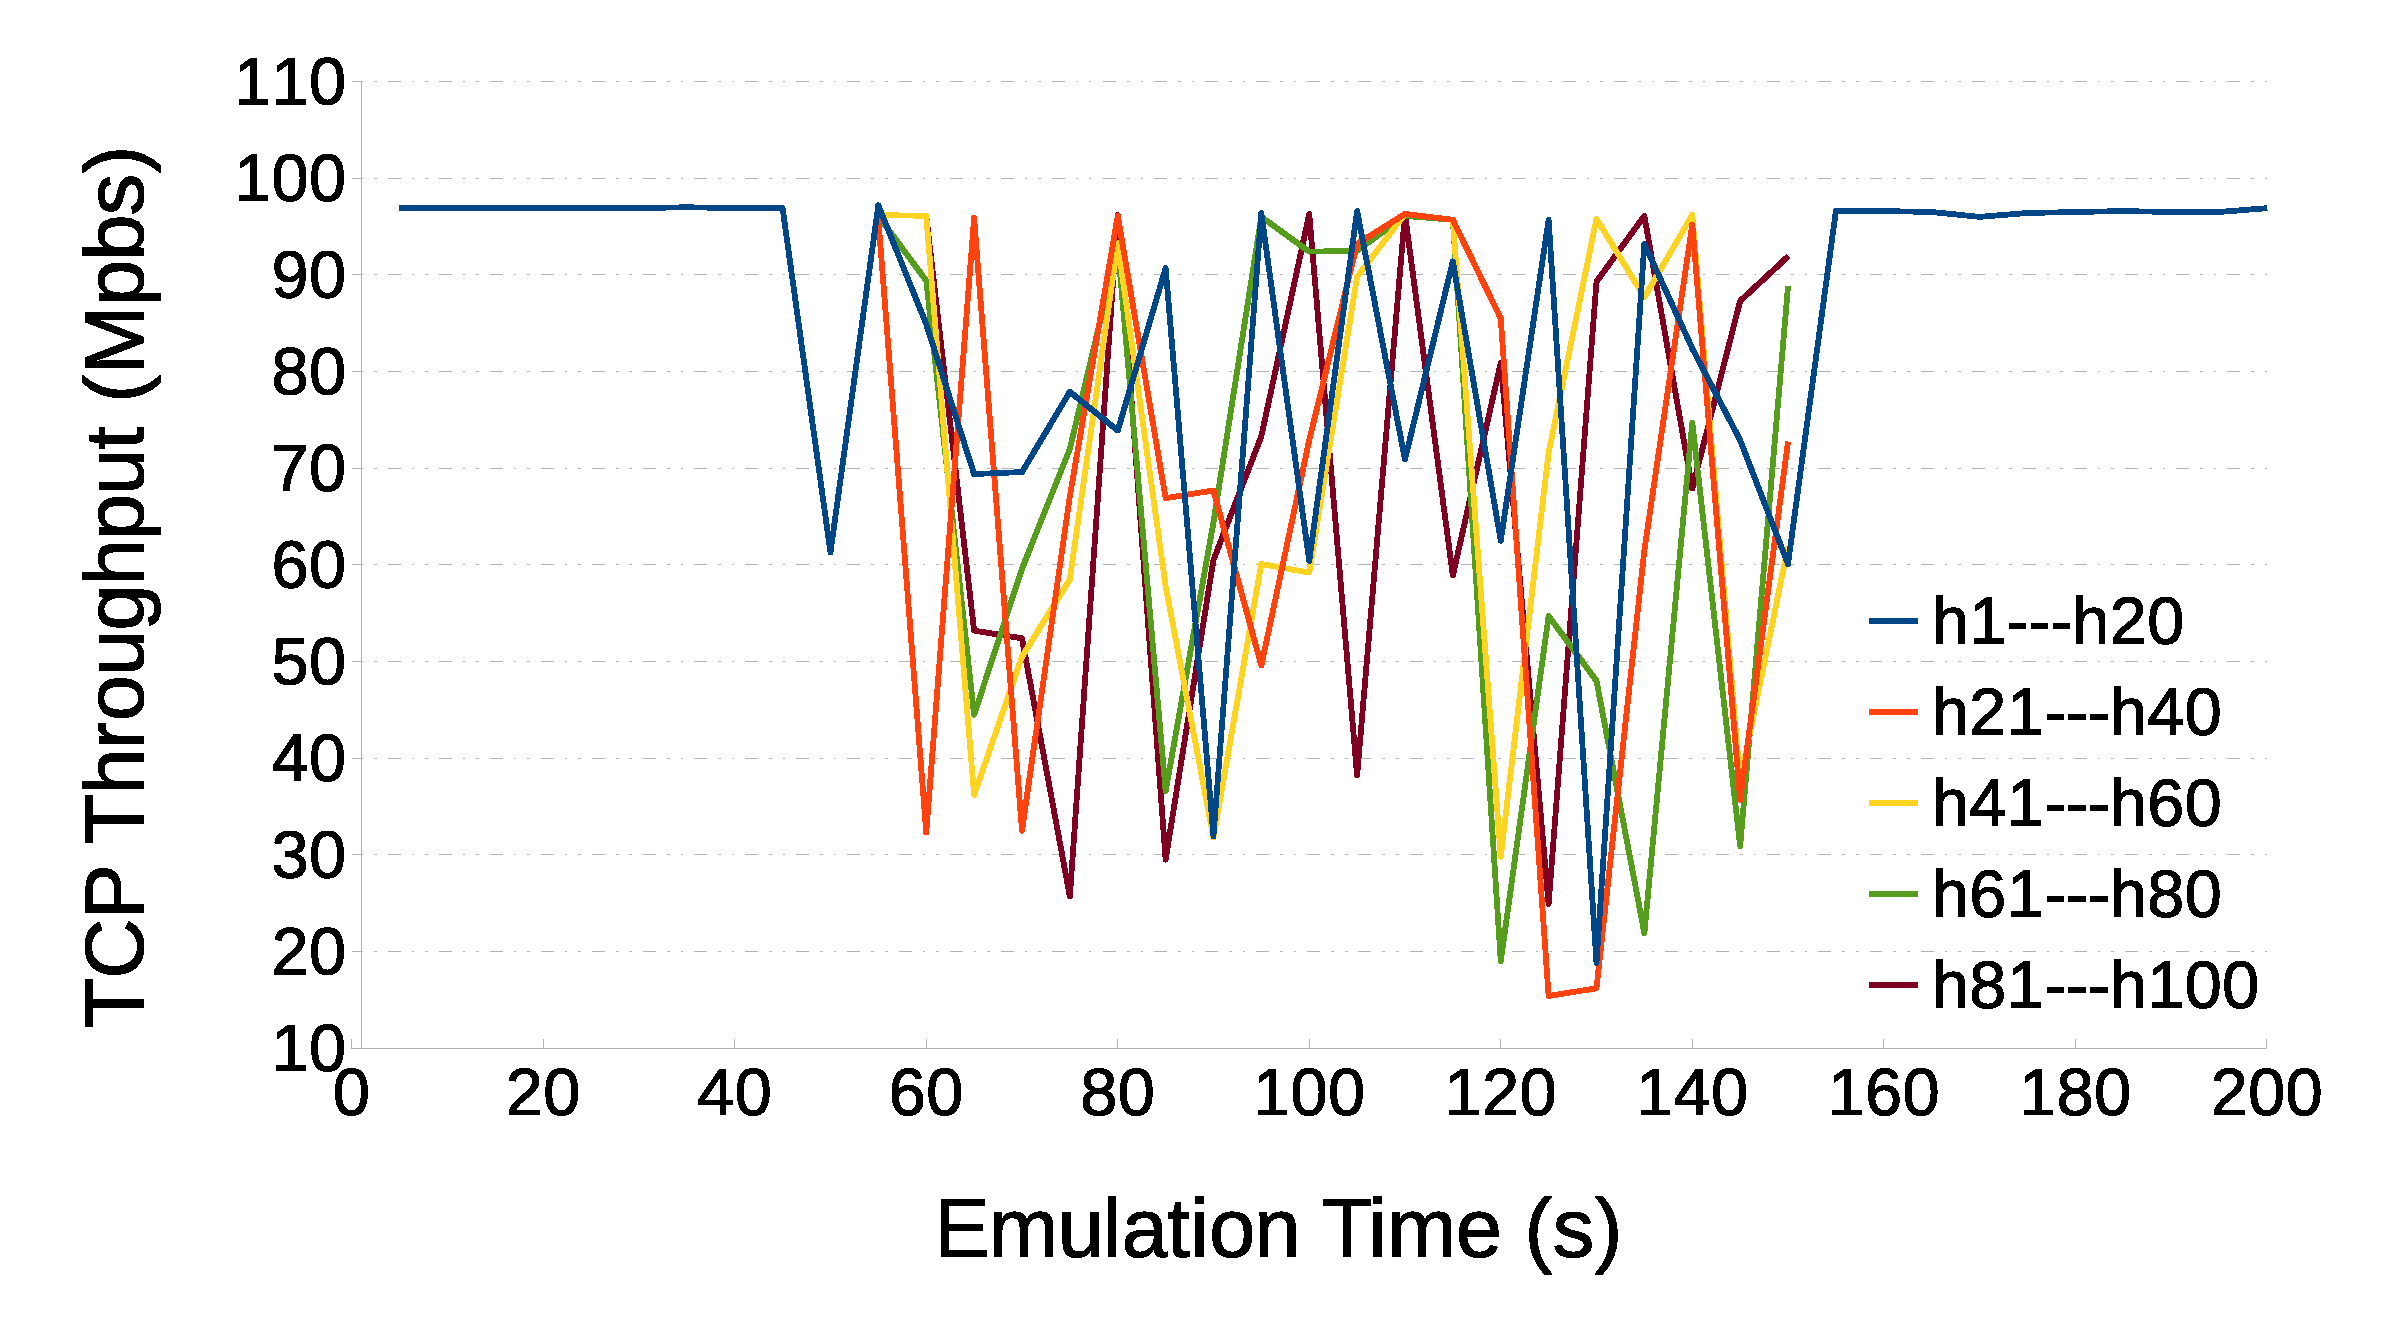
\epsfig{file=VirtualTime/figures/5FlowsNoVT.eps, width=0.45\textwidth}}
    \label{VT:Fig:5FlowsNoVT}}
    \subfigure[TCP Throughput with Adaptive Time Dilation]{\epsfig{file=VirtualTime/figures/5FlowsAdaptiveVT.eps, width=0.45\textwidth}
    \label{VT:Fig:5FlowsAdaptiveVT}}
    \\
    \subfigure[TCP Throughput with Fixed Time Dilation (11)]{\epsfig{file=VirtualTime/figures/5FlowsFixedVT.eps, width=0.45\textwidth}
    \label{VT:Fig:5FlowsFixedVT}}
    \subfigure[TDF Trace: Adaptive Virtual Time Scheduling]{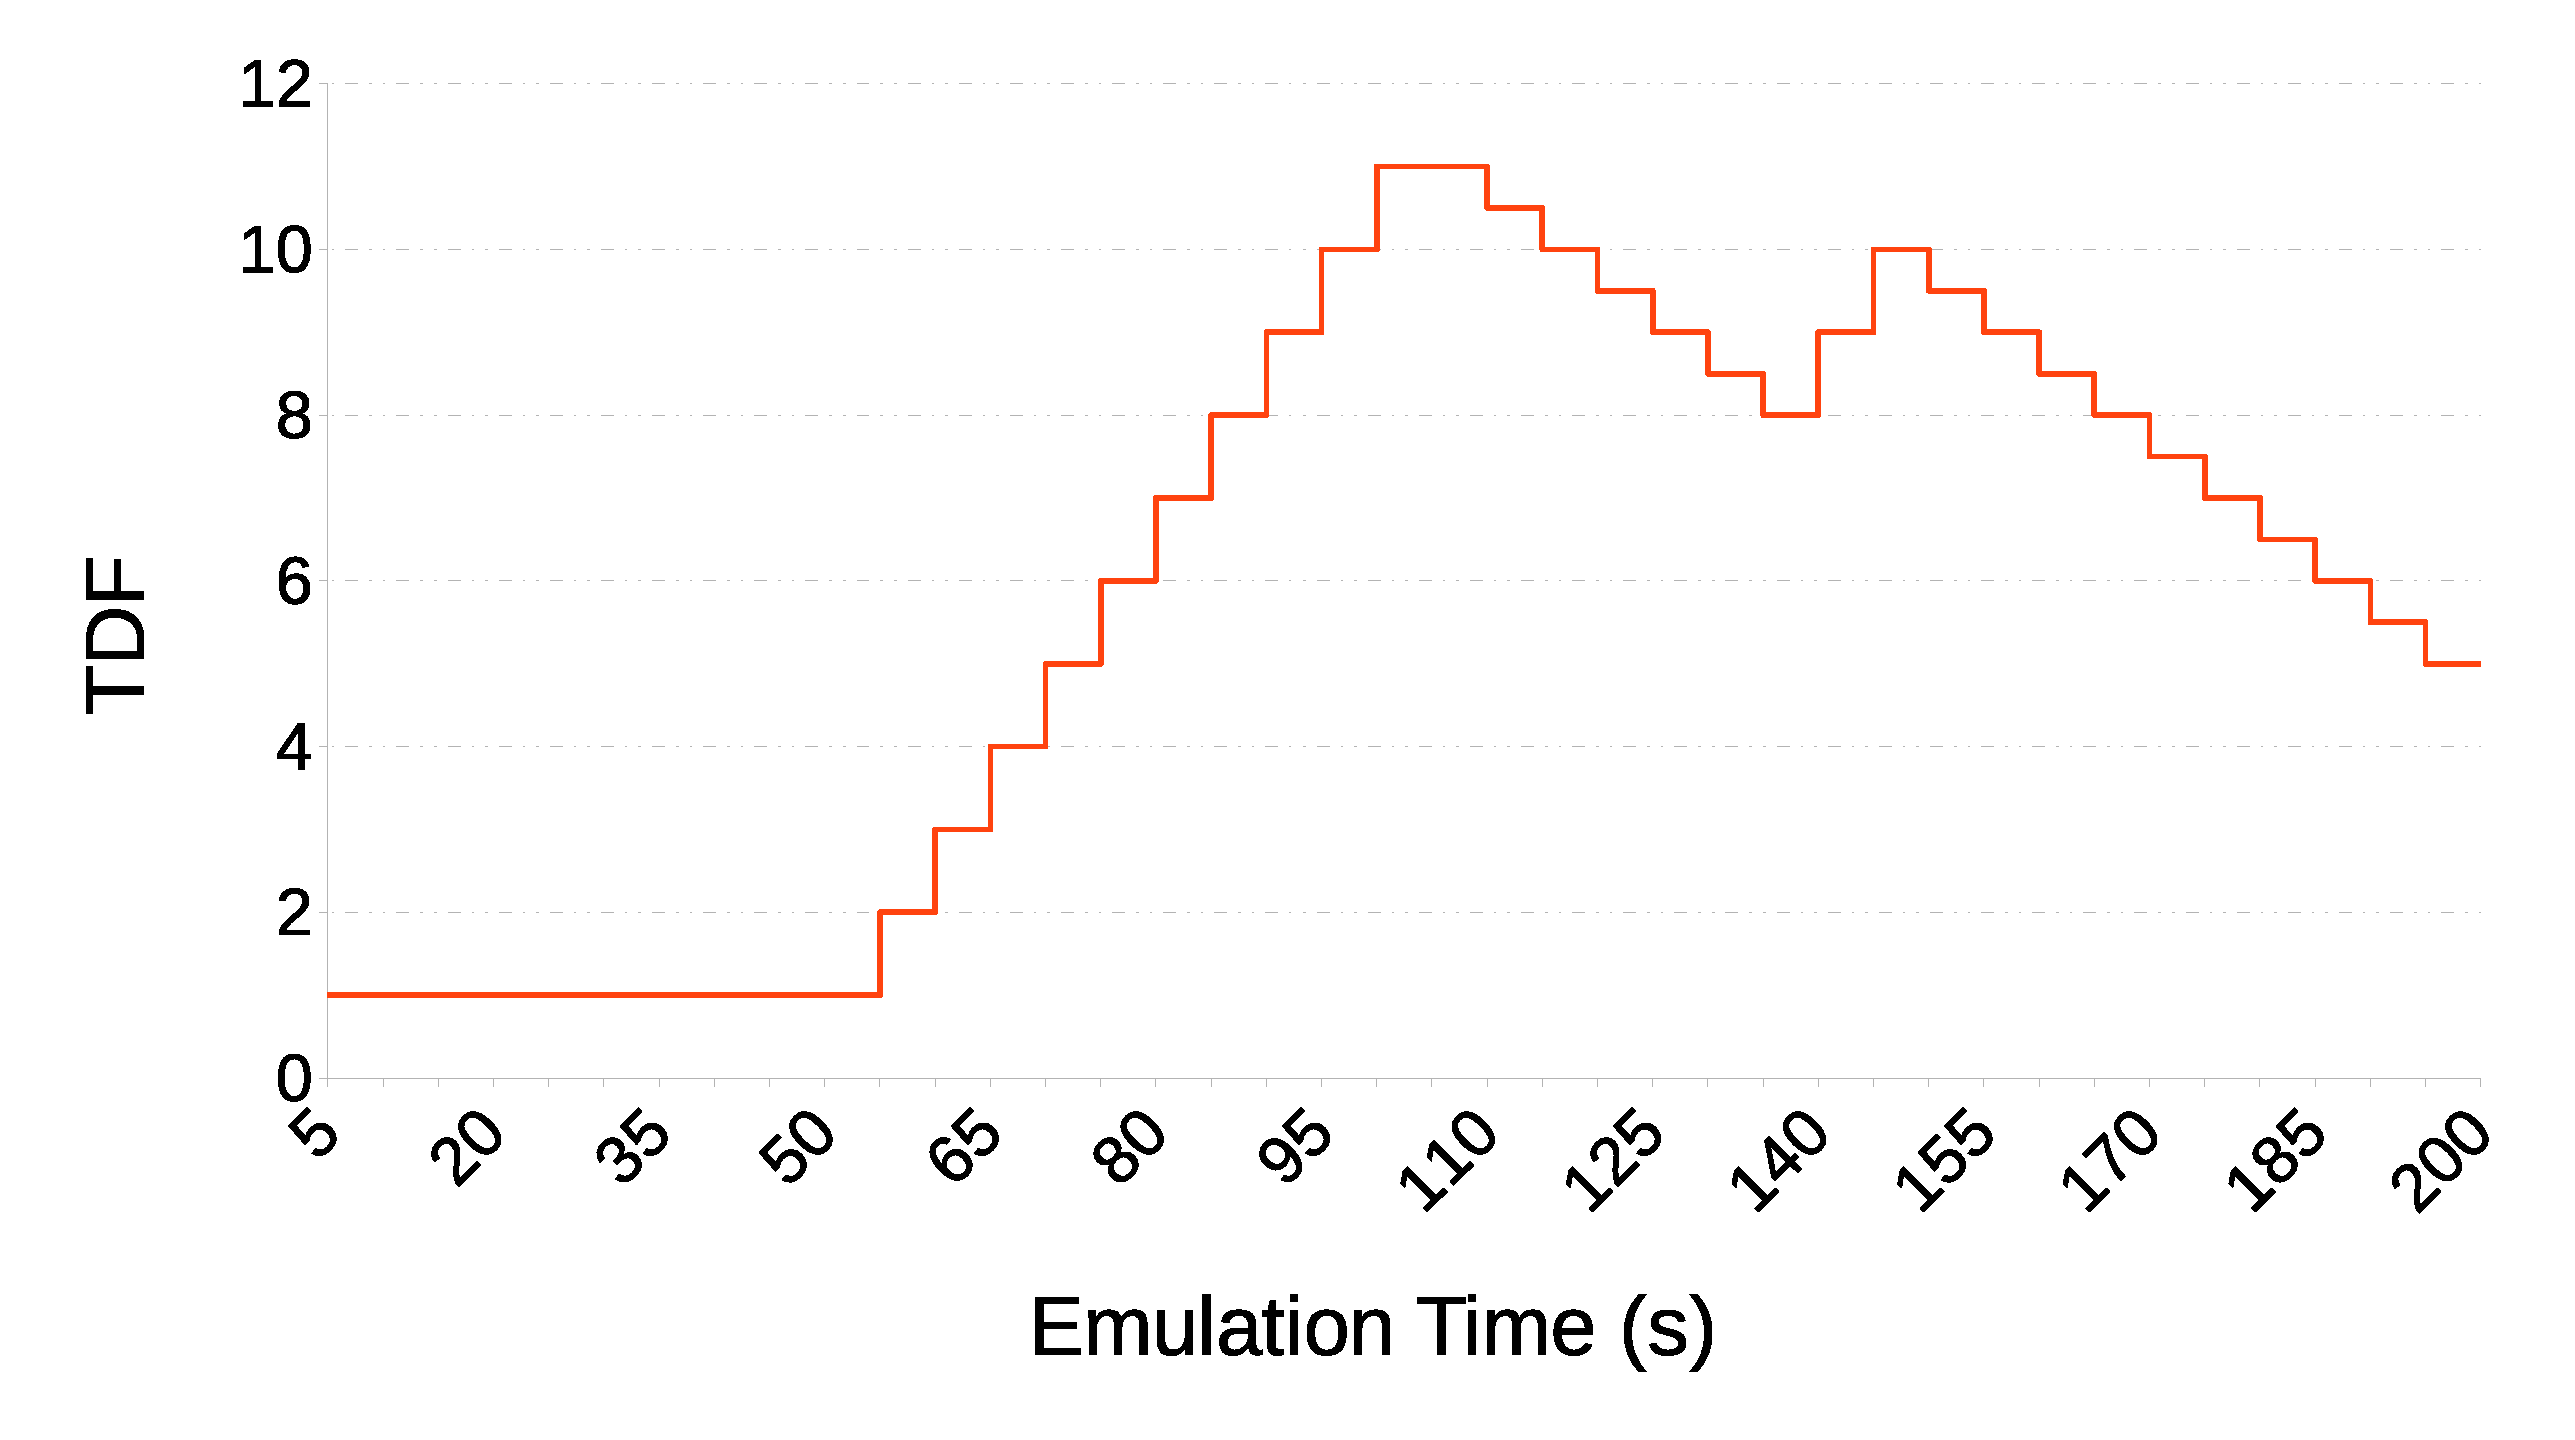
\epsfig{file=VirtualTime/figures/5FlowsHistoryTDF.eps, width=0.45\textwidth}
    \label{VT:Fig:HistoryTDF}}
    \caption{Adaptive Virtual Time Scheduling Evaluation}
    \label{VT:Fig:Adaptive}
\end{figure}

\begin{table*}[t]
    \centering
    \caption{Comparison of Emulation Execution Time}
    \begin{tabular}{lccc} 
        \hline
        \hline
        & No Virtual Time & Adaptive Virtual Time & Fixed Virtual Time \\ 
        \hline
        Running Time (s)  & 240.730 & 1332.242 & 2434.910 \\ 
        Average TDF & 1.000 & 5.900 & 11.000 \\ 
        %Slow Down Ratio & 1.204 & 5.534 & 10.115 \\
        Slow Down Ratio & 1.000 & 5.534 & 10.115 \\
        %\hline
        %AVG. CPU\% & 31.968 & 28.287 & 20.376 \\ 
        %\hline
        %STDEV. CPU\% & 10.915 & 7.175 & 4.173 \\ 
        \hline
    \end{tabular}
    \label{VT:Tab:CompareRunTime}
\end{table*}

\Subsection{System Overhead}
Our virtual time system introduces overhead with the following two reasons:
(1) the computation cost in Algorithm~\ref{VT:Alg:VirtualTimeKeeping} and
(2) the pauses of emulation when changing containers' TDFs.
We measured both types of overhead and report the results in Table~\ref{VT:Tab:Overhead}.

First, we invoked both non-dilated and dilated \texttt{gettimeofday} 10,000,000 times from a user space application.
The average overhead for one dilated \texttt{gettimeofday} is 0.013 microseconds.
We then used \texttt{strace} to count the number of invocations for \texttt{gettimeofday} in a 60-second \texttt{iperf3} run on both the server and the client.
The total overhead is 18,145 microseconds after tracing 1,397,829 calls, which is about 0.03\% of the 60-second experiment. 
Actually, \texttt{iperf3} intensively invokes \texttt{gettimeofday},
because its timer is designed to exhaustively inquiry the OS time.
The overhead amount will be even less for many other network applications.
We also repeatedly changed a process's TDF 10,000,000 times using another test program.
The average pause time was 0.063 microseconds, which is reasonably small.
Since the number of TDF changes issued by the current adaptive TDF scheduling algorithm
is a few orders of magnitude less than the number of calls to \texttt{gettimeofday}
(e.g., only 14 TDF transitions occurred per host over the period of 1,332 seconds in the earlier adaptive TDF experiment), that overhead is also negligible.

\begin{table*}[t]
    \centering
    \caption{Lightweight Virtual Time System: Overhead of System Calls}
    \begin{tabular}{lccc}
        \hline
        \hline
        & No Virtual Time & Virtual Time & Avg Overhead / System Call \\%& Overhead Rate in E  \\ 
        \hline
        \texttt{gettimeofday}  & 0.0532 $\mu$s & 0.0661 $\mu$s & 0.0129 $\mu$s\\% & $3.0 \times 10^{-4}$\\ 
        \texttt{setTDF} & 0  & 0.0628 $\mu$s & 0.0628 $\mu$s\\% & $3.65\times 10^{-9}$ \\ 
        \hline
    \end{tabular}
    \label{VT:Tab:Overhead}
\end{table*}


